\Rank{A問題}
\MonN{43}{基本公式の確認}\par\nopagebreak
\begin{sisin}
絶対屈折率が$n$の媒質中では，波長および光速は$\dfrac{\lambda}{n}\U{m}$, $\dfrac{c}{n}\U{m/s}$になる．

臨界角については，式を覚える必要はない．屈折光が存在する場合について屈折の法則を立式し，その式を元に屈折光が存在しない条件を考えればよい．

(5)の回折格子の干渉条件$d\sin\theta=m\lambda$はしっかり覚えておこう．明線の「次数」とは，干渉条件の式$d\sin\theta=m\lambda$の$m$の値のことを言う（正確には，中心位置を0次として，外側へ1次，2次，$\cdots\cdots$の明線という）．
\end{sisin}
\KaiHead
\begin{komon}
\ko{1} $\dfrac{3.0\times 10^8}{1.5}=2.0\times 10^8\U{m/s}$\hspace*{\fill}\Ans
\ko{2} 求める絶対屈折率を$n$とする．真空の絶対屈折率は1であるから，
       \[1\cdot\sin 60^\circ=n\sin 30^\circ\]
       よって，
       \[n=\sqrt{3}\Ans\]
\ko{3} 求める相対屈折率は，
       \[\frac{2.0}{1.5}=1.33\cdots\fallingdotseq 1.3\Ans\]
\ko{4} 入射角を$\theta$，屈折角を$\varphi$とする．屈折の法則より，
       \[\sin\varphi=2.0\sin\theta\]
       である．屈折光が存在せず全反射するためには，この値が1以上であればよいので，
       \[\sin\varphi=2.0\sin\theta\geqq 1\]
       を満たす入射角$\theta$では全反射が起きる．よって，臨界角は
       \[2.0\sin\theta=1\]
       を満たす角であり，
       \[\theta=30^\circ\Ans\]
\ko{5} 回折格子の格子定数を$d\U{m}$とすると，
       \[d\sin 30^\circ=1\times(600\times 10^{-9})\]
       であるから，
       \[d=2\times(600\times 10^{-9})=1.2\times 10^{-6}\U{m}\]
       ゆえに$1\U{m}$あたりの格子の本数は，
       \[\frac{1}{d}\fallingdotseq 8.3\times 10^{5}\,[個]\Ans\]
\end{komon}

\Rank{B問題}
\MonN{44}{波の性質}\par\nopagebreak
\begin{sisin}
ホイヘンスの原理および回折現象に関する説明文である．この問題に書かれていることは常識として覚えておこう．また，ホイヘンスの原理を用いた屈折の法則の導出方法も併せて確認しておくこと．
\end{sisin}
\KaiHead
\begin{komon}
\ko{1} 素元波
\ko{2} 球面
\ko{3} ホイヘンス
\ko{4} 回折
\ko{5} 波長
\ko{6} 音波
\end{komon}
\begin{chuu}
音波と光波では波長が全く異なる．音波の場合，音速が$340\U{m/s}$，人間の耳の可聴領域がおよそ$20\U{Hz}\sim 20\U{kHz}$程度であるから，その波長はおおよそ$17\U{m}\sim 1.7\U{cm}$程度である．これに対して可視光は波長が$380\U{nm}\sim 780\U{nm}$程度である．我々が日常生活で目にする物体は音波の波長程度の大きさであり，可視光の波長に比べると遥かに大きいため，光波では回折は起きず，音波では回折は起きやすい．そのため，物陰は光が回り込めずに暗い「影」になるが，音は物陰であっても比較的よく聞こえる．
\end{chuu}

\MonN{45}{屈折の法則}\par\nopagebreak
\begin{sisin}
本問の場合は二つの境界面があるので，それぞれに対して屈折の法則を立てる必要がある．真空と媒質$\mathrm{B}$の間に対して直接，屈折の法則を立てることはできないことに注意．また，(2)については媒質$\mathrm{B}$の絶対屈折率を元に計算しよう．

(3)については，媒質$\mathrm{B}$と$\mathrm{A}$の境界面に対する入射角および媒質$\mathrm{A}$中への屈折角を適当な文字で置き，(1)と同様に二つの屈折の法則の式を立てて考える．真空中へ出ていかないための条件式はもちろんだが，媒質$\mathrm{B}$よりも媒質$\mathrm{A}$の屈折率の方が小さいから，入射角によっては媒質$\mathrm{A}$, $\mathrm{B}$の境界面で全反射が起こりうる．よって，媒質$\mathrm{A}$の中に屈折光が存在するための条件も考える必要があることに注意．
\end{sisin}
\KaiHead
\begin{komon}
\ko{1} 真空の絶対屈折率が1であることに注意して，真空・媒質$\mathrm{A}$の境界面，および媒質$\mathrm{A}$, $\mathrm{B}$の境界面のそれぞれに対して屈折の法則より立式すると，
       \[n_\mathrm{A}\sin 45^\circ=1\cdot\sin 60^\circ\]
       \[n_\mathrm{B}\sin 30^\circ=n_\mathrm{A}\sin 45^\circ\]
       である．この二式を解いて，
       \[n_\mathrm{A}=\frac{\sqrt{6}}{2},\hspace{4mm} n_\mathrm{B}=\sqrt{3}\Ans\]
\ko{2} 媒質$\mathrm{B}$の絶対屈折率は$n_\mathrm{B}=\sqrt{3}$であるから，媒質$\mathrm{B}$中での光の速さは，
       \[\frac{3.0\times 10^8}{\sqrt{3}}\fallingdotseq 1.7\times 10^8\U{m/s}\Ans\]
\ko{3} 媒質$\mathrm{B}$と$\mathrm{A}$の境界面に対する入射角を$\theta$，媒質$\mathrm{A}$中への屈折角を$\varphi$とし，さらに真空中への屈折角を$\alpha$とおく．真空中への入射角は$\varphi$となる．
       \begin{center}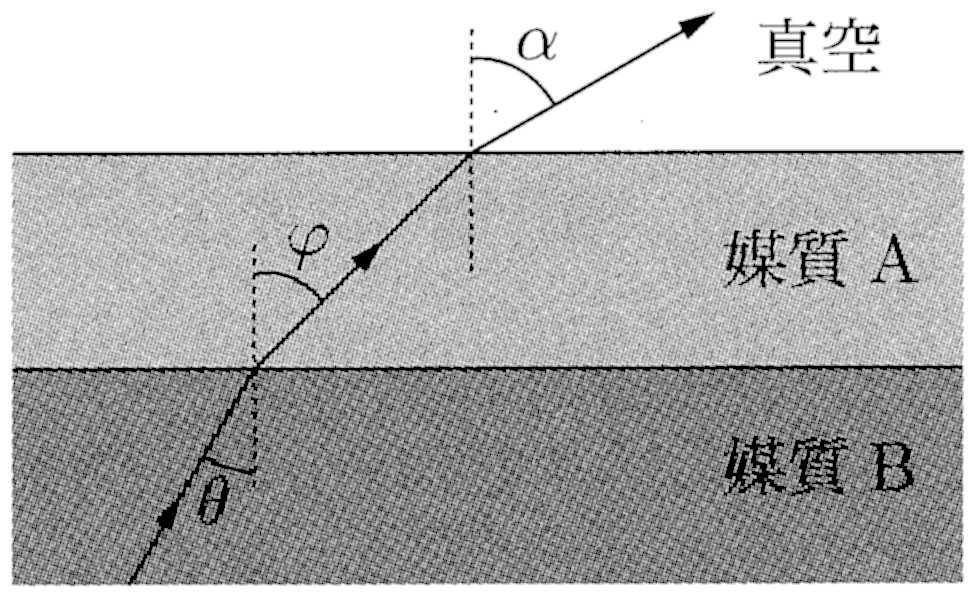
\includegraphics[keepaspectratio,width=62mm]{fig/ch18_ex_refract_ans.png}\end{center}
       各境界面に対して屈折の法則より式を立てると，
       \[n_\mathrm{B}\sin\theta=n_\mathrm{A}\sin\varphi=1\cdot\sin\alpha\]
       であり，
       \[\sin\alpha=n_\mathrm{B}\sin\theta\]
       となる．光が媒質$\mathrm{A}$と真空との境界面ですべて反射されて全反射になるためには，この式を満たす角度$\alpha$が存在しなければよいので，
       \[n_\mathrm{B}\sin\theta\geqq 1\]
       であればよい．また，少なくとも媒質$\mathrm{A}$の中に進まなければ媒質$\mathrm{A}$と真空との間の全反射を考えることができないので，媒質$\mathrm{A}$中へ光が進むために角度$\varphi$が存在することが必要である．ゆえに，
       \[\sin\varphi=\frac{n_\mathrm{B}}{n_\mathrm{A}}\sin\theta<1\]
       が必要である．以上2式を整理して，
       \[\frac{1}{n_\mathrm{B}}\leqq\sin\theta<\frac{n_\mathrm{A}}{n_\mathrm{B}}\]
       であるから，(1)の値を代入して，
       \[\frac{\sqrt{3}}{3}\leqq\sin\theta<\frac{\sqrt{2}}{2}\Ans\]
\end{komon}

\MonN{46}{水中の光源を隠す円板の半径}\par\nopagebreak
\begin{sisin}
空気の屈折率よりも水の屈折率の方が大きいから，水から空気に光が抜けようとするときには，入射角が大きい場合には全反射を起こしうる．よって，全反射が起こらない部分（角度$\varphi$が小さい範囲）について覆いをかぶせてしまえば，空気側からは光源が絶対に見えないことになる．
\end{sisin}
\KaiHead
\begin{komon}
\ko{1} 角度$\varphi$方向に光源から出た光は水面に対して入射角$\varphi$で入射する．これが空気中へ屈折角$\theta$で出ていったとすると，空気と水との境界面において屈折の法則より，
       \[\sin\theta=n\sin\varphi\]
       が成り立つ．屈折角$\theta$が存在しなければ全反射が起こるので，
       \[\sin\theta=n\sin\varphi\geqq 1\]
       であればよい．よって，
       \[\sin\varphi\geqq\frac{1}{n}\Ans\]
\ko{2} 逆に，$\sin\varphi_0=\dfrac{1}{n}$を満たす角度$\varphi_0$よりも小さい角度$\varphi$の範囲では屈折光が空気中へと出てしまうので，この部分を円板で覆い隠せばよい．
       \begin{center}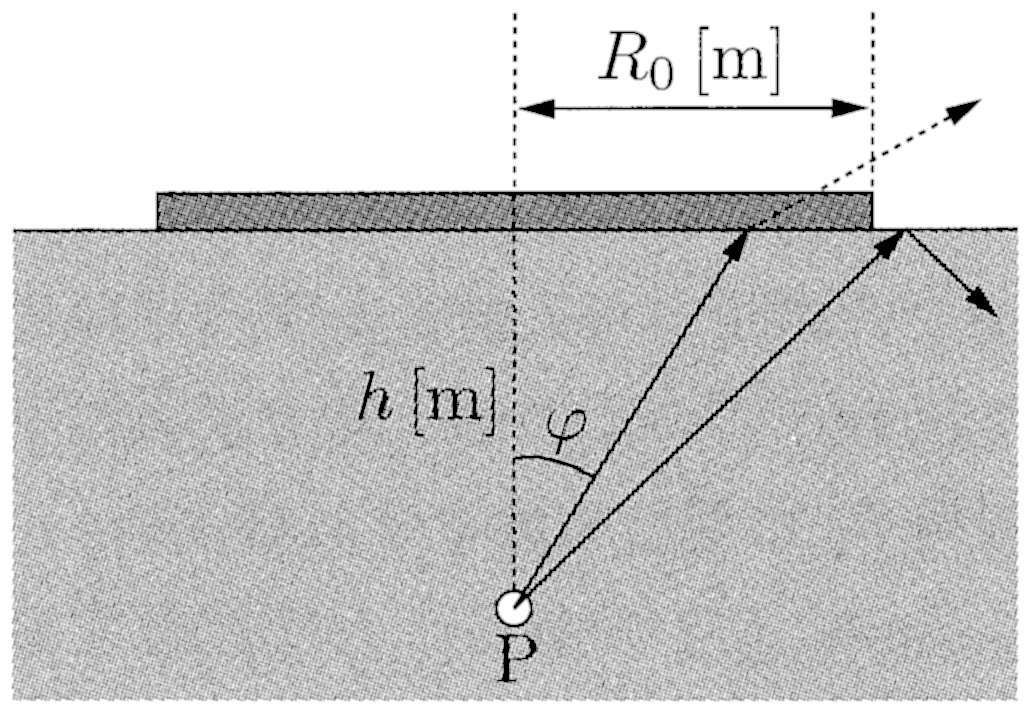
\includegraphics[keepaspectratio,width=62mm]{fig/ch18_p45_disk_ans.png}\end{center}
       ゆえに，
       \[R_0=h\tan\varphi_0\]
       であり，$\sin\varphi_0=\dfrac{1}{n}$より$\cos\varphi_0=\sqrt{1-\dfrac{1}{n^2}}$,
       $\tan\varphi_0=\dfrac{1}{\sqrt{n^2-1}}$であるから，
       \[R_0=\frac{h}{\sqrt{n^2-1}}\U{m}\Ans\]
\end{komon}

\MonN{47}{光ファイバーの原理}\par\nopagebreak
\begin{sisin}
光ファイバーについて考える典型問題である．屈折の法則を組み合わせていけばよい問題．ひとつずつ考えていくこと．
\end{sisin}
\KaiHead
\begin{komon}
\ko{1} $\mathrm{O_1}$点に対して屈折の法則を用いて，
       \[n_1\sin\theta_2=\sin\theta_1\Ans\]
\ko{2} 同様に，$\mathrm{O_2}$点に対して屈折の法則を適用して，
       \[n_1\sin\theta_3=n_2\sin\theta_4\Ans\]
\ko{3} $\theta_2$, $\theta_3$の間には$\theta_2+\theta_3=90^\circ$の関係が成立するので，
       \[\sin^2\theta_2+\sin^2\theta_3=\sin^2\theta_2+\sin^2(90^\circ-\theta_2)\]
       \[=\sin^2\theta_2+\cos^2\theta_2=1\]
       である．これに(1), (2)から得られる
       \[\sin\theta_2=\frac{\sin\theta_1}{n_1},\hspace{4mm}\sin\theta_3=\frac{n_2}{n_1}\sin\theta_4\]
       を代入すると，
       \[\left(\frac{\sin\theta_1}{n_1}\right)^2+\left(\frac{n_2}{n_1}\sin\theta_4\right)^2=1\]
       である．これを整理して，
       \[\sin^2\theta_1+n_2^2\sin^2\theta_4=n_1^2\Ans\]
\ko{4} $\mathrm{O_2}$点で全反射を起こせば反射角$\theta_3$で円柱\MARU{1}内に跳ね返り，その後，角度$\theta_3$での全反射を繰り返していく．$\mathrm{O_2}$点で全反射を起こすためには$\theta_4$が存在しなければよいので，(3)式を変形して
       \[\sin^2\theta_4=\frac{1}{n_2^2}\left(n_1^2-\sin^2\theta_1\right)\geqq 1\]
       であればよい．これより，
       \[n_2\leqq\sqrt{n_1^2-\sin^2\theta_1}\]
       \[\Leftrightarrow\ n_1\geqq\sqrt{n_2^2+\sin^2\theta_1}\Ans\]
\ko{5} 円柱\MARU{1}の側面から入射したすべての光が反射を繰り返して伝わっていくには，(4)で求めた不等号がすべての入射角$\theta_1$に対して成立すればよい．

       $0\leqq\sin\theta_1\leqq 1$であることに注意すると，(4)の条件式が必ず満たされるためには$\sin\theta_1=1$のときに(4)の不等号が成立すればよいので
       \[n_2\leqq\sqrt{n_1^2-1}\]
       であればよい．これを整理して，
       \[n_1^2-n_2^2\geqq 1\Ans\]
\end{komon}
\begin{chuu}
$\mathrm{O_1}$点での屈折では屈折率の大きいものへ波が進行するため，必ず屈折光が存在し，全反射はしない．
\end{chuu}
